% !TEX TS-program = pdflatex
% !TEX encoding = UTF-8 Unicode

\documentclass{beamer}
% for handouts: \documentclass[handout]{beamer}

%\setbeamertemplate{background canvas}[vertical shading][bottom=white,top=structure.fg!25]
% or whatever

\usetheme[compress]{Amsterdam}
%\setbeamertemplate{headline}{}
%\setbeamertemplate{footline}{}
%\setbeamersize{text margin left=0.5cm}
  
\usepackage[english]{babel}
\usepackage{listings}
\usepackage{geometry}
\usepackage{hyperref}

\usepackage{color}
\usepackage[T1]{fontenc}
\usepackage[utf8]{inputenc}
\usepackage{lmodern}


\usepackage{tikz}
\usetikzlibrary{shapes,arrows}

\usepackage{multicol}
\lstset{
basicstyle=\scriptsize\ttfamily,
columns=flexible,
breaklines=true,
numbers=left,
%stepsize=1,
numberstyle=\tiny,
backgroundcolor=\color[rgb]{0.85,0.90,1}
}


\begin{document}

\title[Big Data and Automated Content Analysis]{\textbf{Big Data and Automated Content Analysis} \\ Week 8 -- Monday \\ »Looking back and froward«}
\author[Damian Trilling]{Damian Trilling \\ ~ \\ \footnotesize{d.c.trilling@uva.nl \\@damian0604} \\ \url{www.damiantrilling.net}}
\date{26 March 2018}
\institute[UvA]{Afdeling Communicatiewetenschap \\Universiteit van Amsterdam}




\tikzstyle{block} = [rectangle, draw, fill=blue!20, 
text width=5em, text centered, rounded corners, minimum height=4em]
\tikzstyle{line} = [draw]
\tikzstyle{pijltje} = [draw, -latex']
\tikzstyle{cloud} = [draw, ellipse,fill=red!20, node distance=3cm,
minimum height=2em, text width=4em, text centered,]

















\begin{frame}{}
\titlepage
\end{frame}

\begin{frame}{Today}
\tableofcontents
\end{frame}




\section{Looking back}
\subsection{Putting the pieces together}
\begin{frame}[plain]{}
Looking back\\
\textbf{Putting the pieces together}
\end{frame}


\begin{frame}{First: Our epistomological underpinnings}
	Computational Social Science
\end{frame}


\begin{frame}{Computational Social Science}
	``It is an approach to social inquiry defined by (1) the use of large, complex datasets, often—though not always— measured in terabytes or petabytes; (2) the frequent involvement of “naturally occurring” social and digital media sources and other electronic databases; (3) the use of computational or algorithmic solutions to generate patterns and inferences from these data; and (4) the applicability to social theory in a variety of domains from the study of mass opinion to public health, from examinations of political events to social movements''
	
	\vskip 0.5 cm
	\tiny{Shah, D. V., Cappella, J. N., \& Neuman, W. R. (2015). Big Data, digital media, and computational social science: Possibilities and perils. T\textit{he ANNALS of the American Academy of Political and Social Science, 659}(1), 6–13. doi:10.1177/0002716215572084}
\end{frame}





\begin{frame}{Computational Social Science}
``[\ldots] the computational social sciences employ the scientific method, complementing descriptive statistics with inferential statistics that seek to identify associations and causality. In other words, they are underpinned by an epistemology wherein the aim is to produce sophisticated statistical models that explain, simulate and predict human life.''

\vskip 0.5 cm
\tiny{Kitchin, R. (2014). Big Data, new epistemologies and paradigm shifts. \textit{Big Data \& Society, 1}(1), 1–12. doi:10.1177/2053951714528481}
\end{frame}


\begin{frame}{Second: Our data}
	content...
\end{frame}




\begin{frame}{Third: Our techniques}
	content...
	\end{frame}




\begin{frame}{Steps of a CSS project}
We learned

\end{frame}

\begin{frame}[plain]
\begin{tikzpicture}[node distance = 3cm, auto]
\node [cloud] (retrieve) {retrieve};
\node [cloud, right of=retrieve] (process) {process and/or enrich};
\node [cloud, right of=process] (analyze) {analyze\\ explain\\ predict};
\node [cloud, right of=analyze] (visualize) {communi-cate\\ visualize};


\path [pijltje] (retrieve)--(process);
\path [pijltje] (process)--(analyze);
\path [pijltje] (analyze)--(visualize);


\node [block, below of = retrieve] (retrievetech) {files\\ APIs\\ scraping};
\node [block, below of= process] (processtech) {NLP\\ sentiment\\ LDA\\ SML};
\node [block, below of=analyze] (analyzetech) {group comparisons; statistical tests and models};
\node [block, below of=visualize] (visualizetech) {visualize and communicate};



\path [pijltje] (retrievetech)--(processtech);
\path [pijltje] (processtech)--(analyzetech);
\path [pijltje] (analyzetech)--(visualizetech);


\node [block, below of = retrievetech, fill=green!20] (retrievepython) {glob\\ json \& csv\\ requests\\ twitter\\ tweepy\\ lxml\\ \ldots};

\node [block, below of = processtech, fill=green!20] (processpython) {nltk\\ gensim\\ scikit-learn \ldots};

\node [block, below of = analyzetech, fill=green!20] (analyzepython) {numpy/scipy\\ pandas\\ statsmodels\\ \ldots};

\node [block, below of = visualizetech, fill=green!20] (visualizepython) {pandas\\ matplotlib\\ seaborn\\ \ldots};





\path [line, dashed] (retrieve)--(retrievetech);
\path [line, dashed] (process)--(processtech);
\path [line, dashed] (analyze)--(analyzetech);
\path [line, dashed] (visualize)--(visualizetech);



\path [line, dashed] (retrievetech)--(retrievepython);
\path [line, dashed] (processtech)--(processpython);
\path [line, dashed] (analyzetech)--(analyzepython);
\path [line, dashed] (visualizetech)--(visualizepython);
\end{tikzpicture}
\end{frame}




%{\setbeamercolor{background canvas}{bg=black}
%\begin{frame}[plain]
%\makebox[\linewidth]{
%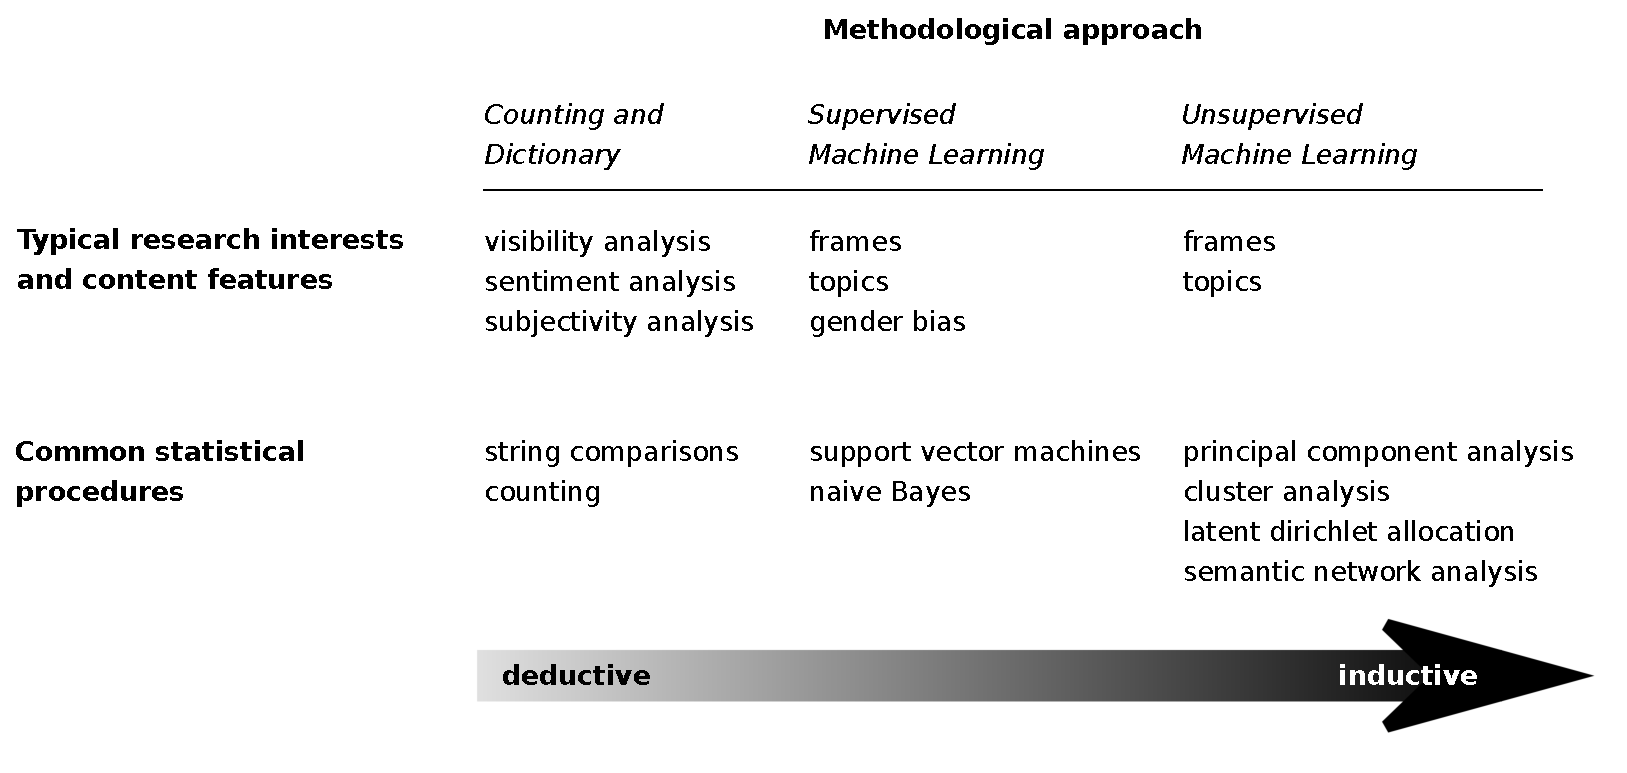
\includegraphics[width=\paperwidth,height=\paperheight,keepaspectratio]{../../pictures//boumanstrilling2016}}
%\end{frame}
%}



%
%\begin{frame}{Some terminology }
%	\begin{columns}[t]
%		\column{.5\textwidth}
%		
%		\begin{block}<1-4>{Supervised machine learning}
%			You have a dataset with both predictor and outcome (independent and dependent variables; features and labels) --- a \emph{labeled} dataset.
%			\onslide<2>{
%				\footnotesize{Think of regression: You measured \texttt{x1}, \texttt{x2}, \texttt{x3} and you want to predict \texttt{y}, which you also measured}}
%		\end{block}
%		
%		\column{.5\textwidth}
%		
%		\begin{block}<3->{Unsupervised machine learning}
%			You have no labels. \onslide<4>{(\footnotesize{You did not measure \texttt{y})}}\\
%			\onslide<5>{\textbf{Again, you already know some techniques to find out how \texttt{x1}, \texttt{x2},\ldots \texttt{x\_i} co-occur from other courses:} \begin{itemize}
%					\item Principal Component Analysis (PCA)
%					\item Cluster analysis
%					\item \ldots
%				\end{itemize}
%			}
%		\end{block}
%		
%	\end{columns}
%	
%\end{frame}
%
%




\subsection{Scaling up}

\begin{frame}[plain]{}
	Looking back\\
	\textbf{Scaling up}
\end{frame}

\begin{frame}{rjbejn}
	functies schrijven
	
	database
	
	
	resusable
	
	terug naar definitie: terabytes?
	
	
\end{frame}



\section{Looking forward}
\subsection{rrkjnjrnkr}
\begin{frame}[plain]{}
Looking forward\\
\textbf{brnrjnkrnjrkn}
\end{frame}




\section{Final steps}

\begin{frame}{HIER NOG EEN SLIDE OVER FINAL PROJECT}
	content...
\end{frame}

\begin{frame}{Next meeting}
\begin{block}{Wednesday}
	Final chance for questions regarding final project (if you don't have any, you don't need to come.)
\end{block}

\begin{block}{Deadline final exam}
Hand in via filesender until Sunday evening, 23.59.
\end{block}


\end{frame}




\end{document}

